\clearpage
\section*{\currfilename}

\begin{figure}[H]
  \begin{center}
    \begin{tikzpicture}[auto, scale=0.85, every node/.style={transform shape}, node distance=1.0cm, >=latex']
      \node[squareblock, minimum height=1cm, minimum width=2cm] (block1){\shortstack[c]{Baseline\\Controller}};
      \node[squareblock, below of=block1, node distance=1.5cm, minimum height=1cm, minimum width=2cm] (block2){\shortstack[c]{Adaptive\\Controller}};
      \matrix[ampersand replacement=\&, row sep=0.5cm, left of=block1,node distance=1cm] (block1in) {
        \node [coordinate] (b1inA) {}; \\
        \node [coordinate] (b1inB) {}; \\
      };
      \matrix[ampersand replacement=\&, row sep=0.5cm, left of=block2,node distance=1cm] (block2in) {
        \node [coordinate] (b2inA) {}; \\
        \node [coordinate] (b2inB) {}; \\
      };
      \node [left of=b2inB, node distance=0.5cm] (2B) {};
      \node [below of=2B, node distance=0.12cm] (2B2) {};
      \node [left of=b2inA, node distance=1.0cm] (2A) {};
      \node [below of=2A, node distance=0.12cm] (2A2) {};
      \node[whitesum,right of=block1, node distance=2.5cm] (sum1) {};
      %\node[squareblock, minimum height=1cm, minimum width=2cm, right of=sum1,node distance=2.5cm] (block3) {Actuators};
      \node[squareblock, minimum height=1cm, minimum width=1.0cm, label=below:{\shortstack[c]{Actuator\\Dynamics}}, right of=sum1,node distance=2.5cm, inner sep= 1mm] (block3) {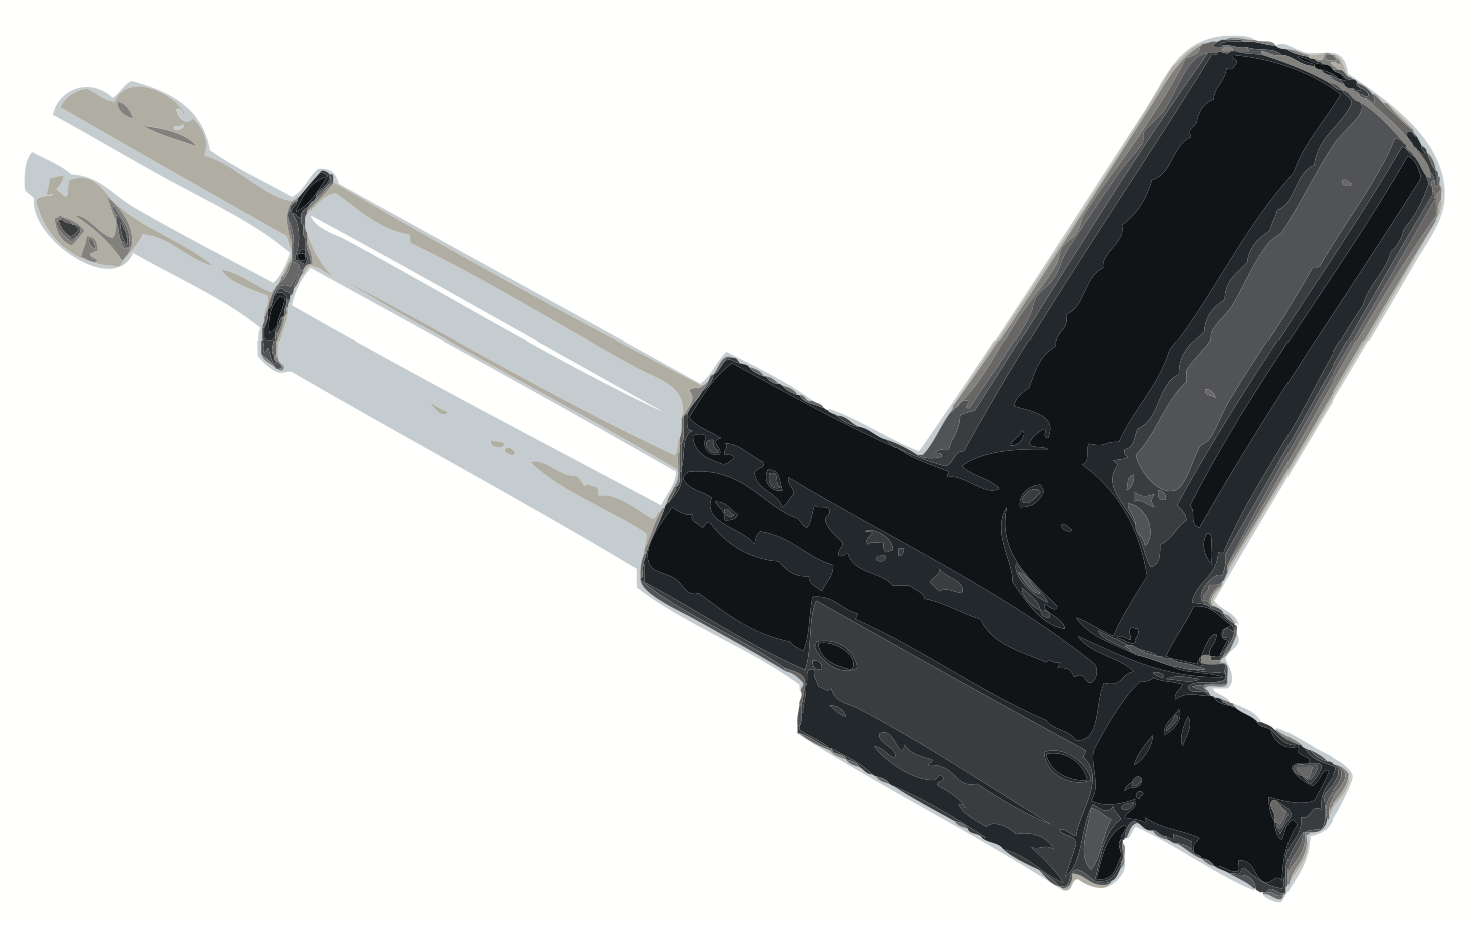
\includegraphics[width=1.6cm]{../fig/actuator_image.png}};
      %\node[squareblock, minimum height=1cm, minimum width=2cm, right of=block3,node distance=3.0cm] (block4) {Plant};
      \node [right of=block3,draw=black, label=below:{\shortstack[c]{6-DOF Nonlinear \\ Equations of Motion}}, anchor=west,node distance=2.0cm, minimum width=2cm, inner sep= 0mm] (block4) {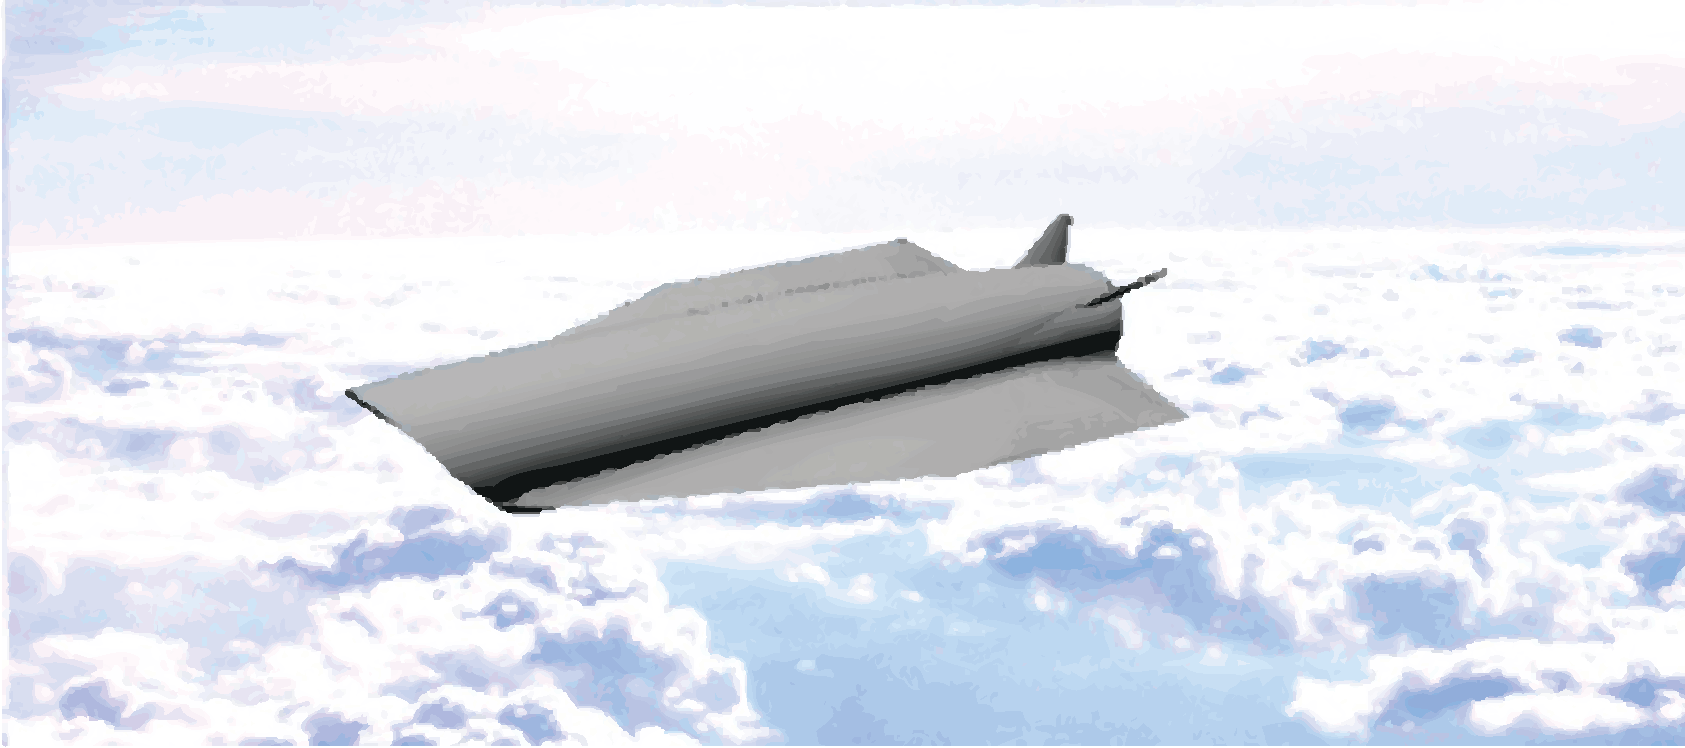
\includegraphics[width=4cm]{../fig/ghvclouds.pdf}};
      %\node[squareblock, minimum height=1cm, minimum width=2cm, right of=block4,node distance=4.0cm] (block5) {Sensors};
      \node[output, right of=block4,node distance=3.5cm] (output1) {};
      \node[input, below of=block2,node distance=1.5cm](input2){};

      \draw [->]  (b1inA) + (-2.5cm,0cm) -> node [pos=0.15]{$z_{\text{cmd}}$}  (b1inA);
      \draw [->]  (b1inB) + (-0.5cm,0cm) -> (b1inB);
      \draw [->]  (b2inA) + (-1cm,0cm) -> (b2inA);
      \draw [->]  (b2inB) + (-2.0cm,0cm) -> node[name=TB,node distance=2.5cm]{} (b2inB);
      \draw[->](block4) --  node[name=yi,pos=0.4]{}(output1);
      \draw[-](yi) |- (input2);
      \draw[-](b1inB) + (-0.5cm,0cm) -- (2B2);
      \draw[-](b1inA) + (-1.0cm,0cm) -- (2A2) ;
      \draw[-] (b2inB) + (-2.0cm,0cm) |- (input2);
      \draw[->](block1) -- node[pos=0.22]{$u_{\text{bl}}$} node[pos=0.9]{$+$} (sum1);
      \draw[->](block2) -| node[pos=0.1]{$u_{\text{ad}}$} node[pos=0.9]{$+$} (sum1);
      \draw[->](sum1) -- (block3);
      \draw[->](block3) -- (block4);
      % \draw[->](block4) -- (block5);
      \begin{pgfonlayer}{background}
        \path (block1 |- block1)+(-2.5,0.7) node (c) {};
        \path (block2 -| block2)+(3.0,-0.7) node (d) {};
        \path[fill=gray!20, draw, dashed] (c) rectangle (d);
      \end{pgfonlayer}
      % \node [below of=block2, node distance = 0.9cm] {Controller};
    \end{tikzpicture}
    \caption{Baseline plus adaptive control block diagram\label{fig.baseplusadaptiveblock}}
  \end{center}
\end{figure}
